\documentclass{frontiersSCNS}
\usepackage{url,hyperref,lineno,microtype,subcaption}
\usepackage[onehalfspacing]{setspace}
\usepackage{float}


\linenumbers

\usepackage[utf8]{inputenc}
\floatplacement{figure}{H}

\def\keyFont{\fontsize{8}{11}\helveticabold }
\def\firstAuthorLast{Villaseñor-Derbez {et~al.}}
\def\Authors{Juan Carlos Villaseñor-Derbez\(^{1,*}\), Eréndira
Aceves-Bueno\(^{1,*}\), Álvin Suarez\(^{2}\), Stuart Fulton\(^{2}\),
Jorge Torre\(^{2}\)}
% Affiliations should be keyed to the author's name with superscript numbers and be listed as follows: Laboratory, Institute, Department, Organization, City, State abbreviation (USA, Canada, Australia), and Country (without detailed address information such as city zip codes or street names).
% If one of the authors has a change of address, list the new address below the correspondence details using a superscript symbol and use the same symbol to indicate the author in the author list.
\def\Address{\(^{1}\)Bren School of Environmental Science and Management, University
of California, Santa Barbara, Santa Barbara, CA,
USA\newline \(^{2}\)Comunidad y Biodiversidad A.C., Guaymas, Mexico}
% The Corresponding Author should be marked with an asterisk
% Provide the exact contact address (this time including street name and city zip code) and email of the corresponding author
\def\corrAuthor{Juan Carlos Villaseñor-Derbez, Bren Hall, University of California,
Santa Barbara, Santa Barbara, CA, 93106}

\def\corrEmail{\href{mailto:jvillasenor@bren.ucsb.edu}{\nolinkurl{jvillasenor@bren.ucsb.edu}}}

\begin{document}
\onecolumn
\firstpage{1}

\title[Community-based marine reserves]{Effectiveness of community-based marine reserves in small-scale
fisheries} 

\author[\firstAuthorLast ]{\Authors} %This field will be automatically populated
\address{} %This field will be automatically populated
\correspondance{} %This field will be automatically populated

\extraAuth{}

\maketitle



\begin{abstract}

Al finalizar revisiones




\medskip
\tiny
 \keyFont{ \section{Keywords:} Marine Protected Areas, Marine Conservation, Small-Scale Fisheries,
Citizen Science, Mexico, Social-Ecological Systems}



\end{abstract}


\textbf{Last update}: 2018-06-29

\clearpage

\section{Introduction}\label{introduction}

Marine ecosystems around the world sustain significant impacts due to
overfishing and unsustainable fishing practices
\citep{halpern_2008-dK,worm_2006-IB,pauly_2005-qV}. In particular,
artisanal fisheries face great challenges since they tend to be hard to
monitor and enforce \citep{costello_2012}. Recent research shows that
combining Territorial Use Rights for Fisheries (TURFs) with no-take
marine reserves (MR) can greatly improve the performance of coastal
fisheries and the health of the local resouces
\citep{costello_2010-Ix,lester_2017}. Commonly known as TURF-Reserves,
these systems increase the benefits of spatial access rights allowing
the maintainance of healthy resources
\citep{afflerbach_2014-HP,lester_2017}.

Marine reserves allow bounded populations to recover by limiting all
extractive activities \citep{halpern_2002}, while the TURF controls the
harvest levels outside the MPA. Although in theory these systems are
successful \citep{costello_2010-Ix}, little empirical evidence evidence
exists of their effectiveness and the drivers of their success
\citep{afflerbach_2014-HP,lester_2017}. The performance of these systems
depends on how environmental and social factors work combined. The
science of marine reserves has largely focused on understanding the
ecological effects of these areas, which include increased biomass,
richness, and densities of organisms within the protected regions,
climate change mitigation, and protection from environmental variability
\citep{lester_2009-Ks,giakoumi_2017-V2,sala_2017-69,roberts_2017-J9,micheli_2012-EU}.
Modelling studies show that fishery benefits of marine reserves depend
on initial stock status and the management under which the fishery
operates, as well as reserve size and the amount of larvae exported from
these \citep{hilborn_2006,krueck_2017-J1}. Other research has focused on
the relationship between socioeconomic and governance structures and
their relationship to reserve effectiveness
\citep{halpern_2013,lpezangarita_2014,mascia_2017-m_}. However, to our
knowledge, no studies exist that evaluate TURF-reserves from both a
social and ecological perspective.

In Mexico many of these marine reserves are created as community-based
marine reserves. Community-based spatial closures occur in other places,
like the \emph{kapu} or \emph{ra'ui} areas in the Pacific Islands
\citep{bohnsack_2004,johannes_2002}. This bottom-up approach increases
compliance and self-enforcement
\citep{gelcich_2015-Gw,espinosaromero_2014-PY,beger_2004-Y8}. However,
without legal recognition these are difficult to enforce and fishers
rely on the exclusive access granted by the TURF. In an effort to bridge
this normative gap, Civil Society Organizations (CSOs) served as the
link between fishers and government, and set out to create a legal
framework that solve this governance issue. In 2014, a new norm was
created, allowing fishers to request the legal recognition of a
community-based reserve under the name of ``Fish Refuge'' \citep{nom}.
These can be implemented as temporal or partial reserves, which can
protect one, some, or all resources within them. Since then, 45 of
community-based marine reserves along the Pacific, Gulf of California,
and Mexican Caribbean coastlines have gained legal recognition, but
their effectiveness has not been reported in the scientific literature.

This work combines causal inference techniques and the social-ecological
systems framework to provide a holistic evaluation of community-based
marine reserves in three coastal communities in Mexico. The objective of
this work is twofold. First, provide a triple bottom line evaluation of
the effectiveness of community-based marine reserves that can inform
similar processes in other countries. And second, evaluate the
effectiveness of TURF-reserves established as Fishing Refugia in Mexico
to identify areas where improvement or adjustment might result in
increased effectiveness. On both cases, we draw from the lessons learned
and provide management recommendations to maximize the effectiveness of
community-based marine reserves in small-scale fisheries.

\section{Materials and Methods}\label{materials-and-methods}

\subsection{Study area}\label{study-area}

We evaluate three TURF-reserves in Mexico (Fig \ref{fig:map}A). The
first one was created by the \emph{Buzos y Pescadores de la Baja
California} fishing cooperative, located in Isla Natividad in the Baja
Peninsula (Fig \ref{fig:map}B). The main fishery in the island is the
spiny lobster (\emph{Panulirus interruptus}), but other resources like
finfish, sea cucumber, read sea urchin, snail, and abalone are also an
important source of income. In 2006, the community decided to implement
two marine reserves within their fishing grounds to protect commercially
important invertebrate species; mainly lobster and abalone. The reserves
obtained legal recognition in 2018, but have been well enforced since
their implementation.

The other two TURF-reserves are located in Maria Elena and Punta
Herrero, in the Yucatan Peninsula (Fig \ref{fig:map}C). Maria Elena is a
fishing camp --visited intermittently during the fishing season--
belonging to the Cozumel fishing cooperative (\emph{SCPP Cozumel});
Punta Herrero is home to the \emph{SCPP José María Azcorra} cooperative.
Their main fishery is the Caribbean spiny lobster (\emph{Panulirus
argus}), but they also target finfish in the off-season. Maria Elena and
Punta Herrero established eight marine reserves in 2012, and four marine
reserves in 2013, respectively. All these reserves are legally
recognized as Fishing Refugia since their creation.

\subsection{Data collection}\label{data-collection}

We use three main sources of information to evaluate these reserves
across the ecological, socioeconomic, and governance dimensions.
Ecological data come from the annual ecological monitoring of reserve
and control areas, carried out by members from each community and
personnel from the Mexican CSO \emph{Comunidad y Biodiversidad}
(\href{www.cobi.org.mx}{COBI}). Trained divers record richness and
abundances of fish and invertebrate species in the reserves and control
sites \citep{fulton_2018}. Size structures are also collected during
fish surveys. We define control sites as regions with habitat
characteristics similar to the corresponding reserves, and that
presumably had a similar probability of being selected as reserves
during the design phase. We focus our evaluation on sites where data are
available for reserve and control sites, before and after the
implementation of the reserve. This provides us with a
Before-After-Control-Impact (\emph{i.e.} BACI) sampling design that
allows us to capture and control for temporal and spatial dynamics
\citep{depalma_2018,ferraro_2006-oW}. BACI designs and causal inference
techniques have proven effective to evaluate marine reserves, as they
allow us to causally attribute observed changes to the intervention
\citep{moland_2013-VP,Villasenor-Derbez_2018}. All sites were surveyed
annually, and at least once before implementation of the reserves. Table
\ref{table:com_sum} shows a summary of the reserves included in this
study.

\begin{figure}
\centering
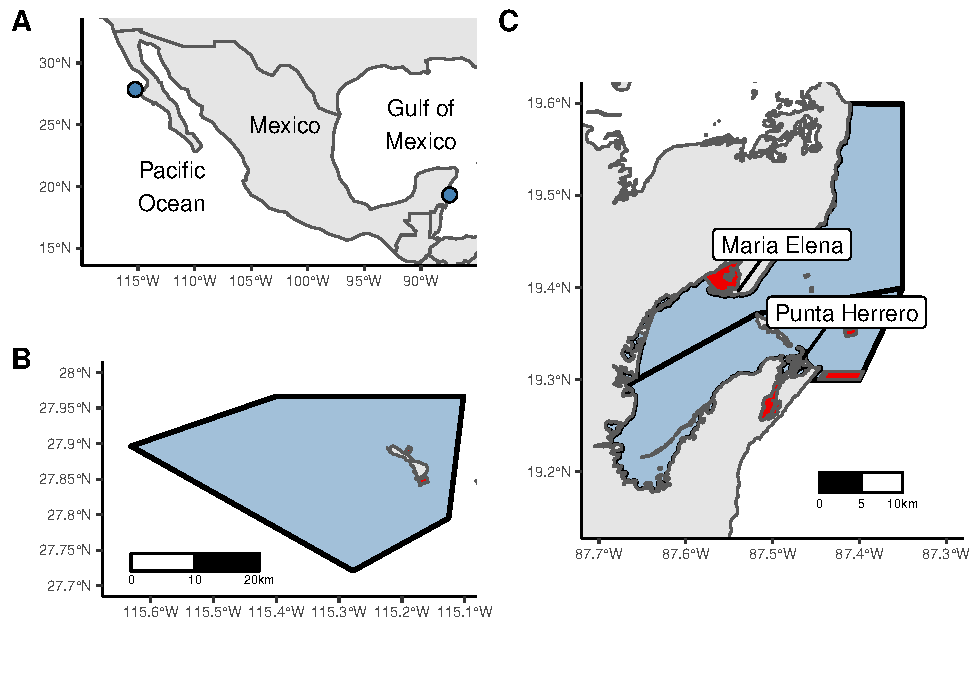
\includegraphics{Villasenor-Derbez_files/figure-latex/unnamed-chunk-1-1.pdf}
\caption{\label{fig:unnamed-chunk-1}\label{fig:map}Location of the three
coastal communities studied (A). Isla Natividad (B) is located off the
Baja California Peninsula, Maria Elena and Punta Herrero (C) are located
in the Yucatan Peninsula. Blue polygons represent the TURFs, and red
polygons the marine reserves.}
\end{figure}

\begin{table}

\caption{\label{tab:unnamed-chunk-2}\label{table:com_sum} Summary of commuity--based marine reserves by community.}
\centering
\begin{tabular}[t]{l|r|r|r|r}
\hline
Community & TURF area ($km^2$) & Reserve area ($km^2$) & Percent as reserves & Year of implementation\\
\hline
Isla Natividad & 889.5 & 1.53 & 0.1720067 & 2006\\
\hline
Maria Elena & 353.1 & 0.10 & 0.0283206 & 2012\\
\hline
Punta Herrero & 299.7 & 0.43 & 0.1434768 & 2013\\
\hline
\end{tabular}
\end{table}

Socioeconomic data come from landing receipts reported to the National
Commission for Aquaculture and Fisheries (\emph{Comisión Nacional de
Acuacultura y Pesca}; CONAPESCA). Data contain monthly lobster landings
(Kg) and revenues (MXP) from 2000 to 2014 for cooperatives with and
without marine reserves(\textbf{Fig S1}). All cooperatives of each
region (\emph{i.e.} Pacific and Caribbean) incorporated in this
analysis, belong to larger Cooperative Federations, and are exposed to
the same markets and institutional frameworks
\citep{mccay_2017-1m,ayer_2018}, making them plausible controls.
Landings and revenues were aggregated at the cooperative-year level, and
revenues were adjusted by the Consumer Price Index for Mexico
\citep{oecd_2017-VV} as:

\begin{equation}
I_t = RI_t\times\frac{CPI_t}{CPI_T}
\label{eqn:cpi}
\end{equation}

Where \(I_t\) represents the adjusted income for year \(t\) as the
product between the reported income for that year and the ratio between
the consumer price index in that year (\(CPI_t\)) to the most recent
year's consumer price index (\(CPI_T\)).

Data for the qualitative analysis of the social-ecological system were
collected at the community--level from official documents used in the
creation and designation of the marine reserves
\citep{dof_website_2012,dof_website_2013,dof_website_2018} and based on
the authors' experience and knowledge of the communities. These include
information on the resource system, the resource units, actors, and the
governance system itself (\textbf{S1 Table}).

\subsection{Data analysis}\label{data-analysis}

We evaluate the effect that marine reserves have had on four ecological
and two socioeconomic indicators (Table \ref{table:indicators}). Recall
that reserves were implemented to protect lobster and other benthic
invertebrates. However, we also use the available fish data to test for
associated co-benefits.

\begin{table}[H]

\caption{\label{tab:unnamed-chunk-3}\label{table:indicators}List of indicators used to evaluate the effectiveness of marine reserves, grouped by category.}
\centering
\begin{tabular}[t]{l|l|l}
\hline
Category & Indicador & Units\\
\hline
Biological & Lobster density & org $\mathrm{m}^{-2}$\\
\hline
Biological & Invertebrate density & org $\mathrm{m}^{-2}$\\
\hline
Biological & Fish biomass & Kg $\mathrm{m}^{-2}$\\
\hline
Biological & Fish density & org $\mathrm{m}^{-2}$\\
\hline
Socioeconomic & Income from target species & M MXP\\
\hline
Socioeconomic & Landings from target species & Metric Tonnes\\
\hline
\end{tabular}
\end{table}

We use a difference-in-differences analysis to evaluate these
indicators. This approach allows us to estimate the effect that the
reserve had by comparing trends across time and treatments (\emph{i.e.}
reserve / control sites \citet{moland_2013-VP,Villasenor-Derbez_2018}).
The analysis of ecological indicators is performed with a multiple
linear regression of the form:

\begin{equation}
I_{itj} = \alpha + \gamma_{t} Year_t + \beta Zone_i + \lambda_{t} Year_t\times Zone_i + \sigma_jSpp_j + \epsilon
\label{eqn:reg_bio}
\end{equation}

Where year-fixed effects are represented by \(\gamma_{it} Year_t\), and
\(\beta Zone_i\) captures the difference between reserve (\(Zone = 1\))
and control (\(Zone = 0\)) sites. The interaction term
\(\lambda_{it} Year_t\times Zone_i\) represents the mean change in the
indicator inside the reserve, for year \(t\), with respect to the year
of implementation in the control site (See Table \ref{table:com_sum}).
When evaluating biomass and densities of the entire benthic or fish
communities, we include \(\sigma_j\) to control for species-fixed
effects.

Socioeconomic indicators are evaluated with a similar approach. Due to
data constrains, we only evaluate socioeconomic data for Isla Natividad
and Maria Elena. Neighboring communities are used as counterfacutals
that allow us to control for unobserved time-invariants. Each
``treated'' community (Isla Natividad and Maria Elena) has three
counterfactual communities.

\begin{equation}
I = \alpha + \gamma_{t} Year_t + \beta Treated_i + \lambda_{t} Year_t\times Treated_i + \sigma_jCom_j +\epsilon
\label{eqn:soc_reg}
\end{equation}

The model interpretation remains as for Eq \ref{eqn:reg_bio}, but in
this case the \(Treated\) dummy variable indicates if the community has
a reserve (\(Treated = 1\)) or not (\(Treated = 0\)) and \(\sigma_jCom\)
captures community-level fixed-effects. These regressions allows us to
make a causal link between the implementation of marine reserves and the
observed trends by accounting for temporal and spatial dynamics
\citep{depalma_2018}. The effect of the reserve is captured by the
\(\lambda_t\) coefficient, and represents the difference observed
between the control site before the implementation of the reserve and
the treated sites at time \(t\) after controlling for other time and
space variations (\emph{i.e.} \(\gamma_t\) and \(\beta\) respectively).
All model coefficients were estimated via ordinary least-squares and
heteroskedastic-robust standard errors \citep{zeileis_2004-7n}. All
analyses were performed in R 3.5.0 and R Studio 1.1.453 \citep{R_2018}.

\section{Results}\label{results}

The following sections present the effect that marine reserves had on
each of the biological and socioeconomic indicators for each coastal
community. Results are presented in terms of the difference through time
and across sites, relative to the control site on the year of
implementation (\emph{i.e.} effect size \(\lambda_t\)). We also provide
an overview of the governance settings of each community, and discuss
how these might be related to the effectiveness and performance of the
reserves.

\subsection{Biological}\label{biological}

Indicators showed ambiguous responses through time for each reserve.
Figure \ref{fig:indicators}A shows positive effect sizes for lobster
densities in Isla Natividad and Punta Herrero during the first years,
but the effect is eroded through time. In the case of Maria Elena,
positive changes were observed in the third and forth year. These
effects are in the order of 0.2 extra organisms \(\mathrm{m}^{-2}\) for
Isla Natividad and Punta Herrero, and 0.01 organisms \(\mathrm{m}^{-2}\)
for Maria Elena, but are not significantly different from zero
(\(p > 0.05\)). The rapid increase observed for changes in lobster
densities for Isla Natividad on the sixth year (\emph{i.e.} 2012) occur
a year after the hypoxia events described by \citet{micheli_2012-EU}
caused mass mortality of organisms. Likewise, no changes were detected
in fish biomass or invertebrate and fish densities
(\ref{fig:indicators}B-D), where effect sizes oscillated around zero
without clear trends. Full tables with model coefficients are presented
in the supplementary materials (\textbf{S2 Table}, \textbf{S3 Table},
\textbf{S4 Table}).

\subsection{Socioeconomic}\label{socioeconomic}

Lobster landings and revenue were only available for Isla Natividad and
Maria Elena (Fig \ref{fig:lobsters}). For all years before
implementation, the effect sizes are close to zero, indicating that the
control and treatment sites have similar pre-treatment trends,
asuggesting that these are plausible controls. However, effect sizes do
not change after the implementation of the reserve. Again, the negative
coefficient observed for Isla Natividad on year 5 correspond to the 2011
hypoxia events. The only positive change observed in lobster landings is
for Isla Natividad in 2014 (\(p < 0.1\)). The three years of
post-implementation data for Maria Elena do not show a significant
effect of the reserve. Isla Natividad shows higher revenues after the
implementation of the reserve, as compared to the control communities.
However, these changes are not significant and are associated to
increased variation. All regression coefficients for each community and
indicator are presented in \textbf{S5 Table}.

\subsection{Governance}\label{governance}

Although we have little information on the social dimension of these
fisheries, we can use the social-ecological systems framework
(\textbf{S1 Table}) to analyze the performance of each governance system
(\textbf{S6 Table}). Our analysis shows that all of the systems analyzed
share similarities in their Governance system which is based on
cooperatives (GS5.2.3.2), with strong rules in use that include
Operational rules (GS6.2), Collective-choice rules (GS6.3),
Constitutional rules (GS6.3), and even Territorial use communal rights
(GS6.1.4.3). However, we identified important differences in terms of
the actors, resource systems, and resource units. Although all
communities show a high level of leadership (A5), the level of trust
(A6.1) is lower in Punta Herrero. In general, the presence and success
of conservation initiatives depends on the incentives of local
communities to maintain a healthy status of the resources they depend
upon \citep{jupiter_2017}. The enabling conditions for conservation seem
to be strongly present in all communities. Due to the clarity of access
rights and isolation, the benefits of conservation directly benefit the
members of the fishing cooperative. These conditions have favored the
development of an efficient community-based enforcement systems.

\clearpage

\begin{figure}
\centering
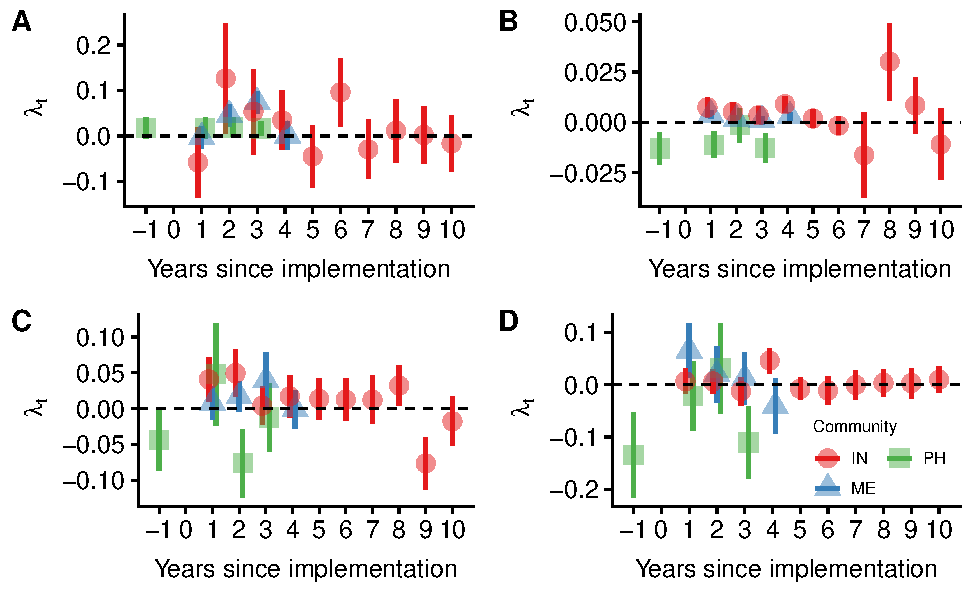
\includegraphics{Villasenor-Derbez_files/figure-latex/unnamed-chunk-4-1.pdf}
\caption{\label{fig:unnamed-chunk-4}\label{fig:indicators}Effect sizes for
marine reserves from Isla Natividad (IN; red cirlcles), Maria Elena (ME;
blue triangles), and Punta Herrero (PH; green squares) for lobster
densities (\emph{Panulirus spp}; A), fish biomass (B), invertebrate
densities (C), and fish densities (D). Plots are ordered by survey type
(left column: invertebrates; right column: fish). Points are jittered
hotizontally to avoid overplotting. Points indicate the effect size, and
errorbars standard errors. Years have been centered to year of
implementation.}
\end{figure}

\begin{figure}
\centering
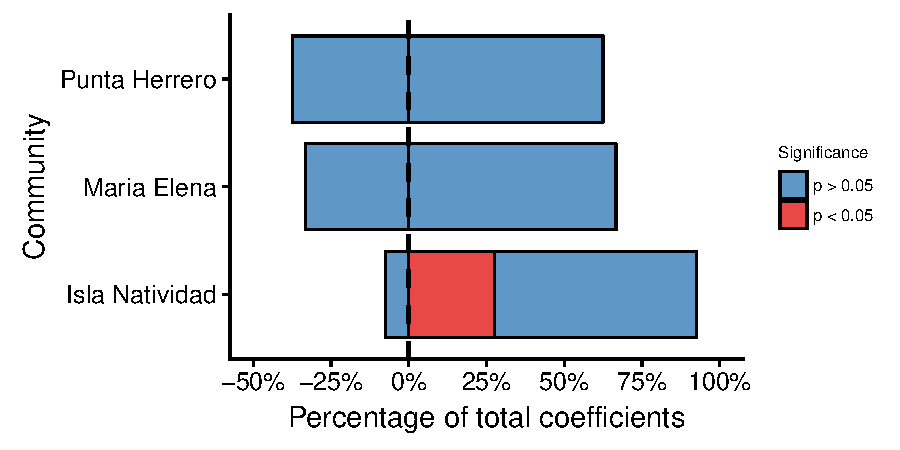
\includegraphics{Villasenor-Derbez_files/figure-latex/unnamed-chunk-6-1.pdf}
\caption{\label{fig:unnamed-chunk-6}\label{fig:lobsters}Effect sizes for
lobster catches (A) and revenues (B) in at Isla Natividad (IN; red
circles) and Maria Elena (ME; blue triangles)}
\end{figure}

\clearpage

\section{Discussion}\label{discussion}

Our results indicate that these TURF-reserves have not increased lobster
densities. Additionally, no co-benefits were identified when using other
ecological indicators other than the previously reported buffering
effect that reserves can have to environmental variability in Isla
Natividad \citep{micheli_2012-EU}. The socioeconomic indicators
pertaining landings and revenues showed little to no change after
reserve implementation. The lack of evidence of the effectiveness of
these reserves is surprising since most of the communities show a
positive perception about their performance and continue to support
their presence \citep{ayer_2018}. Analyzing the shortcomings of our
study and understanding the social-ecological context in which these
communities and their reserves operate might provide insights to this
question.

Some works evaluate marine reserves by performing inside-outside
\citep{guidetti_2014-8Z,friedlander_2017-oI,rodriguez_2017-PD} or
before-after comparisons \citep{betti_2017-lq}. The first approach does
not address temporal variability, and the second can not distinguish
between the temporal trends in a reserve and the entire system
\citep{depalma_2018}. Our approach to evaluate the temporal and spatial
changes provides a more robust measure of reserve effectiveness.
However, this method assumes control sites are a plausible
counterfactual for treated sites. This supposed that treated sites would
have followed the same trend as control sites, had the reserves not been
implemented. Nonetheless, overall trends for each site don't show any
significant increases, supporting our findings of lack of change in the
indicators used (\textbf{S2 Figure}, \textbf{S3 Figure}, \textbf{S4
Figure}, \textbf{S5 Figure}, \textbf{S6 Figure}).

Literature shows that age and enforcement are important factors that
influence reserve effectiveness \citep{edgar_2014-UO}. Isla Natividad
has the oldest reserve, and our SES analysis suggests that all
communities have a well-established community-based enforcement system.
With these characteristics, one would expect the reserves to be
effective. Maria Elena and Punta Herrero are relatively young reserves
(\emph{i.e.} \textless{} 5 years old); other community-based marine
reserves in tropical ecosystems may take up to six years to show a
spillover effect \citep{dasilva_2015-zX}.

Another key condition for effectiveness is reserve size
\citep{edgar_2014-UO}, and the lack of effectiveness can perhaps be
attributed to reserves being too small. Previous research has shown that
reserves in Isla Natividad yield fishery benefits for the abalone
fishery \citep{rossetto_2015-V0}. Abalone are less mobile than lobsters,
and perhaps the reserves provide enough protection to these sesile
invertebrates, but not lobsters. Design principles developed by
\citet{green_2017} for marine reserves in the Caribbean state that
reserves ``should be more than twice the size of the home range of
adults and juveniles'', and suggest that reserves seeking to protect
spiny lobsters should have at least 14 km across. Furthermore, may favor
implementation of reserves that pose low fishing costs due to their
small size or location. Our analysis of economic data supports this, as
neither landings nor revenues showed the expected short-term costs
associated to the first years of reserve implementation
\citep{ovando_2016-Wg}. Small reserves can serve as a way to
self-regulate the spatial distribution of fishing effort

Even if reserves had appropriate sizes and were placed in optimal
locations, there are other plausible explanations for the observed
patterns. For instance, marine reserves are only likely to provide
fisheries benefits if initial population sizes are low and the fishery
is poorly managed \citep{hilborn_2006}. Both lobster fisheries were, at
some point, certified by the Marine Stewardship Council
\citep{prezramrez_2016-J1}. Additionally, lobster fisheries are managed
via species-specific minimum catch sizes, seasonal closures, protection
of ``berried'' females, and escapement windows where traps are allowed
\cite{dof_website_1993}. It is uncertain whether such a well-managed
fishery will experience additional benefits from marine reserves.

While reserves fail to provide fishery benefits, there are a number of
additional ecological, fisheries, and social benefits. Marine reserves
provide protection to a wider range of species and vulnerable habitat,
like coral reefs. These sites can serve as an insurance against
environmental shocks or mistakes in fisheries management
\citep{hilborn_2004,hilborn_2006,micheli_2012-EU}. Self-regulation of
fishing effort (\emph{i.e.} reduction in harvest) can serve as a way to
compensate for future declines associated to environmental variation
\citep{finkbeiner_2018}. Embarking in a marine conservation project can
bring the community together, which promotes social cohesion and builds
social capital. Furthermore, showing commitment to marine conservation
allows fishers to have greater bargaining power and leverage over
fisheries management.

Community-based marine reserves in small-scale fisheries can be helpful
conservation and fishery management tools when appropriately
implemented. Lessons learned from these cases can guide implementation
of community-based marine reserves elsewhere. For the particular case of
the marine reserves that we evaluate, the possibility of expanding
reserves or merging existing polygons into larger areas should be
evaluated and proposed to the communities. At the broader scale, having
full community support surely represents an advantage, but it is
important for marine reserves to meet essential design principles such
as size and placement. Community-based marine reserves might have more
benefits that result from indirect effects of the reserves, which should
be taken into account when evaluating the outcomes of similar projects.

\section*{Conflict of Interest Statement}

The authors declare that the research was conducted in the absence of
any commercial or financial relationships that could be construed as a
potential conflict of interest.

\section*{Author Contributions}

JC and EA analyzed and interpreted data, discussed the results, and
wrote the first draft. AS, SF and JT discussed the results and edited
the manuscript.

\section*{Funding}

JCVD: CONACyT (Beca de Posgrados en el extranjero, CVU 669403) and the
Latin American Fisheries Fellowship.

AS, SF and JT Walton Family Foundation, Summit Foundation, and Oak
Foundation.

\section*{Acknowledgments}

The authors wish to acknowledge Arturo Hernández and Imelda Amador for
contributions on the governance data, as well as pre-processing
biological data. This study would have not been possible without the
effort by members of the communities here mentioned, who collected the
biological data.

\section*{Supplemental Data}

\href{http://home.frontiersin.org/about/author-guidelines#SupplementaryMaterial}{Supplementary Material}
should be uploaded separately on submission, if there are Supplementary
Figures, please include the caption in the same file as the figure.
LaTeX Supplementary Material templates can be found in the Frontiers
LaTeX folder

\paragraph*{S1 Figure}
\label{S1_Figure}

Map of control and treated sites in A and control and treated landings
in B

\paragraph*{S2 Figure}
\label{S2_Figure}

Time series of biological indicators for IN

\paragraph*{S3 Figure}
\label{S3_Figure}

Time series of biological indicators for ME

\paragraph*{S4 Figure}
\label{S4_Figure}

Time series of biological indicators for PH

\paragraph*{S5 Figure}
\label{S5_Figure}

Time series of economic indicators for ME

\paragraph*{S6 Figure}
\label{S6_Figure}

Time series of economic indicators for PH

\paragraph*{S1 Table}
\label{S1_Table}

Coefficient estimates for biological indicators in Isla Natividad

\paragraph*{S2 Table}
\label{S2_Table}

Coefficient estimates for biological indicators in Maria Elena

\paragraph*{S3 Table}
\label{S3_Table}

Coefficient estimates for biological indicators in Punta Herrero

\paragraph*{S4 Table}
\label{S4_Table}

Coefficient estimates for economic indicators

\bibliographystyle{frontiersinSCNS_ENG_HUMS}\bibliography{references}

\section*{Figure captions}



\end{document}
